% ══════════════════════════════════════════════════════════════════════════════
% Addendum_Auditoria_QLoRA.tex
%
% Fragmento LaTeX (NO es un documento standalone — sin \documentclass ni
% \begin{document}). Pensado para copiarse/pegarse o \input{}-earse dentro de
% Conclusions_Avance6.tex, justo después de la sección "Limitaciones
% metodológicas" (o antes de "Trabajo futuro"). Usa los mismos macros que ese
% documento (\ghref, \code) — deben estar definidos en el preámbulo del
% archivo donde se inserte este fragmento.
%
% Contenido: (1) resultado de la ablación del filtro de drawdown
% (qlora_no_drawdown, 2026-06-17) y (2) verificación de que el periodo de
% prueba es posterior al corte de pre-entrenamiento de Qwen2.5 (descarta
% memorización como explicación de la accuracy alta).
%
% Fuentes: docs/qlora/AUDIT_QLORA_88PCT.md §10 (addendum), langgraph/
% optimization-results.ipynb Part 8, langgraph/optimization/qlora/results/
% qlora_no_drawdown/result.json
% ══════════════════════════════════════════════════════════════════════════════

% ── Ablación del filtro de drawdown ─────────────────────────────────────────
\section{Ablaci\'on del filtro de \textit{drawdown}}
\label{sec:ablation-drawdown}

La auditor\'ia adversarial (\ghref{docs/qlora/AUDIT\_QLORA\_88PCT.md}{\code{AUDIT\_QLORA\_88PCT.md}}, \S2) se\~nal\'o que el filtro de \textit{drawdown-before-profit} del etiquetador --- que descarta cualquier muestra cuyo SL se hubiera activado antes que el TP dentro de la ventana de 24 velas --- introduce sesgo de supervivencia: solo se etiquetan trayectorias que \textit{funcionaron} en retrospectiva. La auditor\'ia predijo que, sin este filtro, la accuracy ca\'er\'ia a 60--70\% sobre datos m\'as ruidosos.

Para cuantificar este efecto se ejecut\'o una ablaci\'on de una sola variable: se reentren\'o el modelo con \textbf{hiperpar\'ametros id\'enticos} a \code{qlora\_cloud} (lr=2e-5, rank=16, alpha=32, 2 \'epocas) sobre un dataset reconstruido sin el filtro de \textit{drawdown} (\code{dataset\_no\_drawdown\_filter.jsonl}, 75,289 muestras vs.\ 56,161 --- un 34.1\% m\'as grande, ya que se retienen trayectorias ``ruidosas pero direccionalmente correctas''). Todos los dem\'as filtros (ADX$\geq$15, volumen$\geq$0.5, R:R$\geq$1.0, \textit{whipsaw}) permanecen sin cambios.

\begin{table}[H]
\centering
\caption{Ablaci\'on del filtro de \textit{drawdown}: mismos hiperpar\'ametros, dataset filtrado vs.\ sin filtro}
\label{tab:ablation-drawdown}
\footnotesize
\begin{tabularx}{\columnwidth}{Xcc}
\toprule
\textbf{M\'etrica} & \textbf{Filtrado} & \textbf{Sin filtro} \\
\midrule
Accuracy (test) & \textbf{88.03\%} & \textbf{84.13\%} \\
Win rate & 61.67\% & 50.55\% \\
Profit factor$^\dagger$ & 12.92 & 4.13 \\
Max drawdown & 12.3\% & 39.7\% \\
Sharpe ratio & 15.79 & 9.40 \\
Train acc.\ (diag.) & 70.5\% & 88.5\% \\
Gap (train$-$test) & $-$17.5pp & $+$4.4pp \\
Muestras evaluadas (N) & 3,000$^\ddagger$ & 11,294 \\
\bottomrule
\end{tabularx}
{\scriptsize $^\dagger$PF circular (TP/SL de hindsight, ver \S\ref{sec:discussion}). $^\ddagger$Sub-muestreo por \textit{stride}; el run sin filtro eval\'ua el test set completo --- los dos N no son id\'enticos, ver caveat metodol\'ogico abajo.}
\end{table}

\begin{figure}[H]
\centering
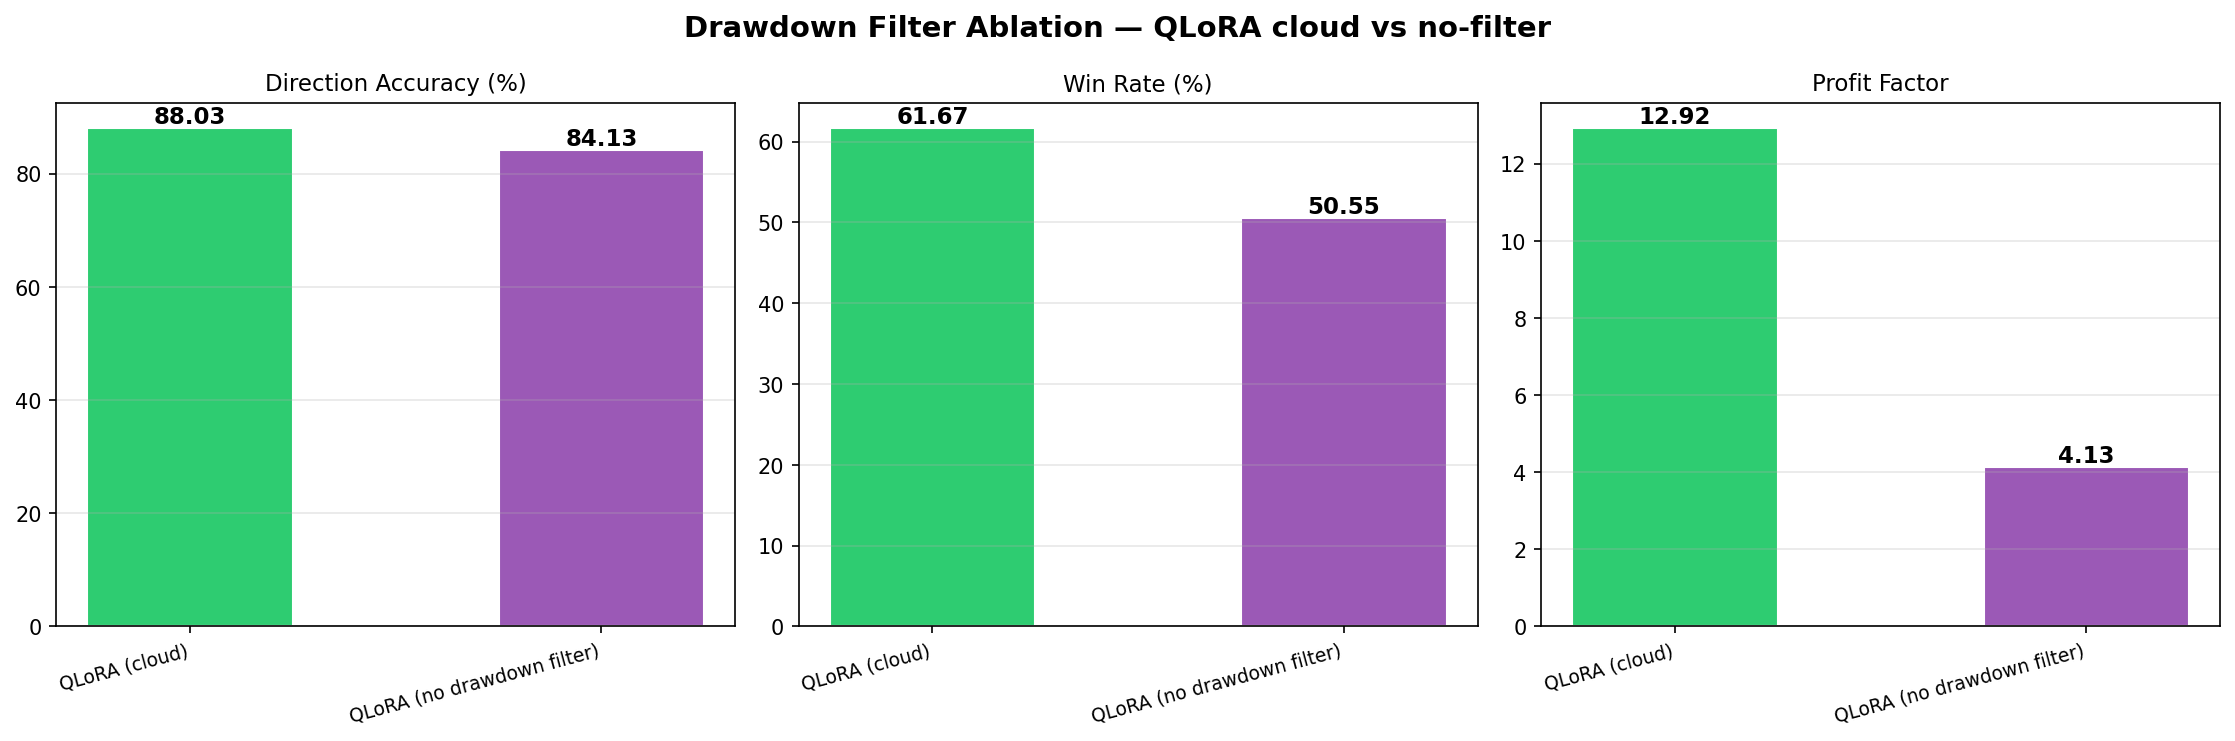
\includegraphics[width=\columnwidth]{figures/fig9_drawdown_ablation.png}
\caption{Ablaci\'on del filtro de \textit{drawdown}: accuracy, win rate y profit factor, mismos hiperpar\'ametros.}
\label{fig:ablation-drawdown}
\end{figure}

\textbf{Hallazgo principal: remover el filtro \emph{reduce} la accuracy} (88.03\%$\rightarrow$84.13\%, $-$3.90pp), no la mejora --- a pesar de entrenar sobre un dataset 34\% m\'as grande. Esto contradice la hip\'otesis original de la auditor\'ia de que el filtro estar\'ia inflando artificialmente el 88.03\% reportado: la evidencia emp\'irica apunta a que el filtro es una \textbf{se\~nal de calidad leg\'itima}, no un artefacto de inflaci\'on.

\textbf{El signo de la brecha train/test se invierte.} \code{qlora\_cloud} tiene gap negativo y saludable ($-$17.5pp, test $>$ train). El modelo sin filtro tiene gap \textbf{positivo} ($+$4.4pp, train $>$ test) --- el patr\'on cl\'asico de sobreajuste. Sin el filtro, el modelo aprende patrones de trades ruidosos que no se sostienen fuera de la muestra de entrenamiento.

\begin{figure}[H]
\centering
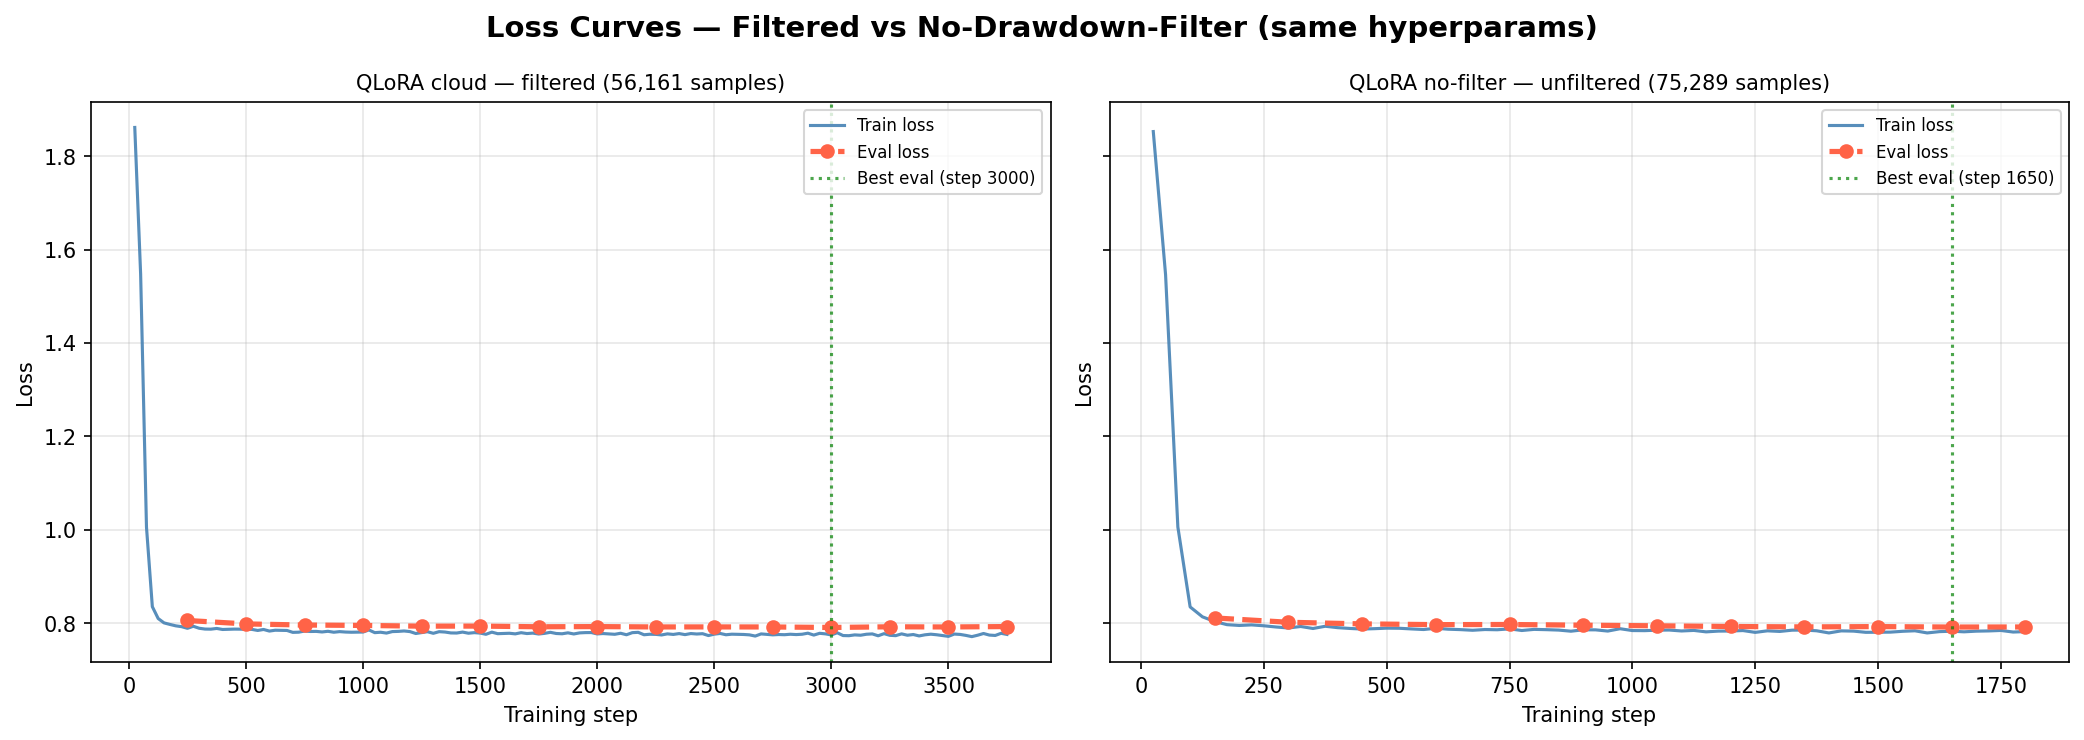
\includegraphics[width=\columnwidth]{figures/fig10_loss_curves_ablation.png}
\caption{Curvas de p\'erdida: filtrado vs.\ sin filtro, mismos hiperpar\'ametros. El run sin filtro detiene el entrenamiento por \textit{early stopping} en el paso 1,800/6,576 (27\% del plan).}
\label{fig:ablation-loss}
\end{figure}

\textbf{Caveat metodol\'ogico.} \code{qlora\_cloud} se eval\'uo sobre un subconjunto estratificado de 3,000 muestras (\code{--max-eval 3000}); el run sin filtro se eval\'uo sobre el test set completo (11,294 muestras, sin \code{--max-eval}). El N mayor en el segundo caso es estad\'isticamente m\'as robusto, pero los dos n\'umeros no provienen exactamente del mismo conjunto de evaluaci\'on --- una comparaci\'on pareada v\'ia \code{align\_results()} (an\'aloga a la prueba de McNemar de \S\ref{sec:discussion}) ser\'ia necesaria para una prueba de significancia estad\'istica rigurosa de esta diferencia de $-$3.90pp.

% ── Verificación de memorización por pre-entrenamiento ──────────────────────
\section{Verificaci\'on: \textquotedblleft memorizaci\'on\textquotedblright\ por pre-entrenamiento}
\label{sec:pretraining-memorization}

Una hip\'otesis adicional considerada --- no cubierta por la auditor\'ia original --- es si Qwen2.5 podr\'ia estar recuperando movimientos de precio hist\'oricos \textbf{memorizados durante su pre-entrenamiento}, en lugar de razonar a partir de los indicadores del prompt. Este ser\'ia un vector de fuga de informaci\'on completamente externo al pipeline de datos/partici\'on/etiquetado ya auditado --- los pesos del modelo mismos ``recordando'' qu\'e ocurri\'o en una fecha y s\'imbolo dados.

Se verificaron las fechas calendario reales de las velas en \code{dataset.jsonl}: el dataset abarca del 23 de noviembre de 2024 al 8 de mayo de 2026. La partici\'on de prueba (el 15\% m\'as reciente) cae aproximadamente entre febrero y mayo de 2026. Los modelos Qwen2.5 reales fueron publicados en septiembre de 2024 con un corte de pre-entrenamiento anterior a esa fecha (Qwen Team, 2024).

\textbf{Veredicto: la memorizaci\'on exacta queda descartada para el conjunto de prueba.} El periodo de prueba es cronol\'ogicamente \textbf{posterior} al corte de conocimiento de Qwen2.5 --- el modelo base no pudo haber memorizado la acci\'on de precio espec\'ifica que se eval\'ua, porque a\'un no exist\'ia cuando el modelo fue pre-entrenado.

\textbf{Caveat --- no completamente cerrado.} Esto solo descarta la memorizaci\'on \textit{exacta} de resultados de este periodo. No descarta un \textit{prior} m\'as difuso --- p.\ ej.\ asociaciones generales pre-entrenadas como ``BTC es un activo de gran capitalizaci\'on y volatilidad comparativamente menor'', o familiaridad con la terminolog\'ia de an\'alisis t\'ecnico (los nombres de las categor\'ias \code{heatmap}/\code{structure}, las convenciones de RSI/ADX) --- que podr\'ian seguir contribuyendo a la ventaja del LLM sobre los modelos ML de \'arbol, de una manera que no es una fuga, sino simplemente un \textit{prior} inicial m\'as rico. Esto es la misma explicaci\'on de ``asimetr\'ia de informaci\'on'' ya planteada en \S\ref{sec:discussion}, ahora acotada: es familiaridad pre-entrenada con \textit{conceptos}, no memorizaci\'on pre-entrenada de \textit{resultados}.

\textbf{Prueba pendiente (no ejecutada a\'un).} Un experimento de oclusi\'on de \textit{features} --- remover \code{heatmap}/\code{structure} (los campos categ\'oricos que los modelos de \'arbol solo ven como enteros ordinales con p\'erdida de informaci\'on) y/o anonimizar el nombre del s\'imbolo del prompt --- permitir\'ia aislar cu\'anto de la brecha de 24pp frente a XGBoost/RF se debe a la codificaci\'on textual categ\'orica versus la capacidad de razonamiento gen\'erica del modelo.
